%===============================================================================
\chapter{Identifica��o de sistemas n�o lineares}
\label{chapter:nlin_si_ident}
%===============================================================================
% idea: Colocar aqui neste capitulo todas as defini��es genericas sobre 
% n�o linearidades. coisas que na� sao relacionadas com o que eu vou fazer, ou que n�o
% sao conseguencia dela.
%
% lineariza��o: Descrever que muitas aplica�oes de identifica��o de sis nonlineares �
% linearizar ele em torno de um ponto. que isso ja eh bom suficiente.
%
% Models: Descrever os tipos de modelos para descrever sistemas nao lineares. Aqui 
% da para escrever bastante coisa. existem muito tipo de modelos para isso.
%
% Algoritmos: aqui vai o algoritmo do aguirre para modelos racionais. Talvez fosse de
% pensar em colcar isso no capitulo com minhas contribui��es? acho que nao .. referencio isso
% no meu capitulo.
%
% Conclus�es: Resumo do que foi visto aqui 
%===============================================================================
%===============================================================================
\section{Conceitos b�sicos}
\label{sec:nlin_si_basic}
%===============================================================================

Existem duas b�sicas limita��es para sistemas linearizados. Primeiro que a lineariza��o
� uma aproxima��o ao redor do ponto de opera��o, ele pode prever apenas o comportamento
nesta localidade do sistema e n�o o comportamento global do sistema. Segundo as din�micas
de sistemas n�o lineares s�o muito mais ricas que as de sistemas lineares. Existem alguns
{\it{essenciais}} fen�menos n�o lineares que n�o conseguem ser descritos ou preditos por
modelos lineares, estes s�o: \cite{khalil}

\renewcommand{\labelitemi}{$\bullet$}
\begin{itemize}

\item Tempo de fuga finito

O estado de um sistema linear inst�vel tende ao infinito na medida que o tempo 
tende ao infinito. Um sistema n�o linear est�vel, entretanto, pode ir para o
infinito em um tempo finito.


\item M�ltiplos pontos de equil�brios isolados

Um sistema linear tem apenas um ponto de equil�brio. Desta forma, este sistema pode
ter apenas um ponto do espa�o de estados que atraem o estado do sistema, independentemente
do estado inicial. Um sistema n�o linear pode ter mais de um ponto de equil�brio isolado. 
Desta forma o estado do sistema pode convergir para um destes equil�brios ou outro,
dependendo do estado inicial do sistema.

\item Ciclos limites

Para um sistema linear e invariante no tempo oscilar ele deve ter um par de autovalores
sobre o eixo imagin�rio, o que � uma condi��o n�o robusta praticamente imposs�vel de manter
na presen�a de perturba��es. Mesmo que isso seja poss�vel de manter, a amplitude da 
oscila��o depender� das condi��es iniciais do sistema. Na vida real, oscila��es est�veis
s�o atingidas com sistemas n�o lineares. Alguns sistemas possuem oscila��es com
amplitude e frequ�ncia constantes, independente das condi��es iniciais. Chama-se isso de
ciclos limites.

\item Sub harm�nicas, harm�nicas ou quase peri�dicas oscila��es

Um sistema linear est�vel sobre uma entrada peri�dica produz uma sa�da na mesma frequ�ncia.
Sistemas n�o lineares alimentados por sinais peri�dicos podem oscilar com frequ�ncias que
podem ser sub m�ltiplos ou m�ltiplos da frequ�ncia de entrada.

\item Caos

Um sistema n�o linear pode ter um espa�o de estados mais complexo que seu comportamento n�o 
pode ser descrito por oscila��es peri�dicas, ou quase peri�dicas oscila��es. Este comportamento
normalmente � conhecido como caos. Alguns destes movimentos ca�ticos exibem comportamento
rand�mico, independentemente da natureza do sistema.

\item M�ltiplos modos de comportamento

� comum para um sistema n�o linear exibir dois ou mais modos de comportamento distintos.
\end{itemize}








Talvez o mais comum uso de sistemas lineares variantes no tempo esta relacionado
a lineariza��o de sistema n�o lineares em torno de uma trajet�ria. Suponha que
o sistema n�o linear � descrito por:

\begin{equation}
\left\{\begin{matrix}
x(k+1) = f(x(k),u(k))+r(x(k),u(k))w(k)\\ 
y(k)  = h(x(k))+m(x(k),u(k))\upsilon (k)
\end{matrix}\right.
\label{eq:nl_linearization_sys}
\end{equation}


%===============================================================================
\section{Modelos para sistemas n�o lineares}
\label{sec:nl_models}
%===============================================================================
% ideia aqui � colocar uma pequena introdu��o sobre modelos.. no mesmo estilo
% que foi para sistemas lineares.

Na se��o (\ref{sec:sys_ident_modelling_choosing}) foi apresentado o conceito de modelos para
sistemas lineares. Nesta se��o ser� apresentado de forma an�loga o conceito de modelos e tipos de
modelos para sistemas n�o lineares. Um problema fundamental referente a modelos parametrizados 
refere-se ao fato do parametro poder ou n�o ser determinado nos valores medidos de entrada e sa�da
dos dados. \cite{glad_ljung}

Na se��o (\ref{sec:nl_models_wiener_hammerstein}) ser� apresentado um dos modelos mais antigos e que
juntamente com o modelo de Voltera (se��o (\ref{sec:nl_models_volterra})) iniciaram o
desenvolvimento dos modelos matem�ticos para sistemas n�o lineares. 

Tamb�m ser� apresentado modelos mais recentes, como as fun��es radiais de base (se��o
(\ref{sec:nl_models_radiais})) derivadas do conceito de redes neurais (\ref{sec:nl_models_neurals}).
Por fim ser� apresentado o conceito de modelos {\it{NARX}} e duas de suas representa��es:
Polinomiais (se��o (\ref{sec:nl_models_narmax_pol})) e Racionais (se��o
(\ref{sec:nl_models_narmax_rat})) que s�o amplamente utilizadas para caracteriza��o de sistemas n�o
lineares, devido entre outros fatores aos algoritmos desenvolvidos e a quantidade de sistemas reais
que podem ser descritos por estes modelos.

Um dos passos mais desafiadores na constru��o de modelos n�o lineares � a escolha da estrutura de
modelo. Quando este modelo � n�o linear, existe uma grande quantidade de op��es e com isso o perigo
de se escolher um modelo desnecessariamente complexo. Isso se baseia no {\it{principio da
parsemonia}} que basicamente detemina que o modelo deve ser o mais simples poss�vel.
\cite{aguirre_maps}

Uma das primeiras raz�es para o desenvolvimento de metodos para a escolha de modelos � a grande
dificuldade de trablhar com modelos muito grandes e complexos. Existe o problema destes modelos
serem numericamente mal condicionados. Existe tamb�m uma convic��o de que estes modelos com muitos
parametros s�o redundantes e poderiam ser removidos do modelo. Um modelo com um n�mero exessivo de
parametros podem exibir dinamicas que n�o s�o observadas no sistema real, desta forma n�o existe
apenas o problema num�rico para estes sistemas, mas tamb�m um problema de din�mica.
\cite{aguirre_jacome}


% ===============================================================================
\subsection{Modelos de Wiener e Hammerstein}
\label{sec:nl_models_wiener_hammerstein}
% Aguirre: 334
% ljung 143
%===============================================================================

Em uma situa��o onde a din�mica do sistema pode ser bem descrita por um sistema linear, 
mas existem algumas n�o linearidades est�ticas atreladas a entrada e/ou a sa�da.
Este ser� o caso de atuadores serem n�o lineares como por exemplo: devido a satura��o, 
ou se o sensor tem caracter�sticas n�o lineares. 

Um modelo com n�o linearidades na entrada � chamado de {\it{modelo de Hammerstein}} e 
para n�o linearidades na sa�da chama-se {\it{modelo de Wiener}}. \cite{ljung}

Considere o sistema apresentado em \eqref{eq:nl_linearization_sys} e o caso de 
Hammerstein, tem-se que a fun��o est�tica n�o linear $f(\cdot)$ pode ser parametrizado
tanto em termos de par�metros f�sicos, como ponto ou n�vel de satura��o, como pode
ser parametrizado por modelo caixa preta.

Na Figura (\ref{fig:nl_models_hammerstein_wiener}) observa-se o diagrama de bloco para os modelos
de Hammerstein e Wiener.


\begin{figure}[htbp]
\center
\scalebox{1} % Change this value to rescale the drawing.
{
	\begin{pspicture}(0,-1.4)(8.949375,1.4)
		\psline[linewidth=0.04cm,arrowsize=0.08cm 2.0,arrowlength=1.4,arrowinset=0.4]{->}(0.0,0.8)(1.2,0.8)
		\psframe[linewidth=0.04,dimen=outer](3.4,1.4)(1.2,0.2)
		\psline[linewidth=0.04cm,arrowsize=0.08cm 2.0,arrowlength=1.4,arrowinset=0.4]{->}(3.4,0.8)(4.6,0.8)
		\psframe[linewidth=0.04,dimen=outer](6.8,1.4)(4.6,0.2)
		\psline[linewidth=0.04cm,arrowsize=0.08cm 2.0,arrowlength=1.4,arrowinset=0.4]{->}(6.8,0.8)(8.0,0.8)
		\psline[linewidth=0.04cm,arrowsize=0.08cm 2.0,arrowlength=1.4,arrowinset=0.4]{->}(0.0,-0.8)(1.2,-0.8)
		\psframe[linewidth=0.04,dimen=outer](3.4,-0.2)(1.2,-1.4)
		\psline[linewidth=0.04cm,arrowsize=0.08cm 2.0,arrowlength=1.4,arrowinset=0.4]{->}(3.4,-0.8)(4.6,-0.8)
		\psframe[linewidth=0.04,dimen=outer](6.8,-0.2)(4.6,-1.4)
		\psline[linewidth=0.04cm,arrowsize=0.08cm 2.0,arrowlength=1.4,arrowinset=0.4]{->}(6.8,-0.8)(8.0,-0.8)
		\usefont{T1}{ptm}{m}{n}
	\rput(0.489375,1.11){u(t)}
	\usefont{T1}{ptm}{m}{n}
	\rput(3.900625,1.11){f(u(t))}
	\usefont{T1}{ptm}{m}{n}
	\rput(7.299375,1.11){y(t)}
	\usefont{T1}{ptm}{m}{n}
	\rput(5.6226563,0.91){Modelo}
	\usefont{T1}{ptm}{m}{n}
	\rput(5.5264063,0.51){Linear}
	\usefont{T1}{ptm}{m}{n}
	\rput(2.2226562,-0.69){Modelo}
	\usefont{T1}{ptm}{m}{n}
	\rput(2.1264062,-1.09){Linear}
	\usefont{T1}{ptm}{m}{n}
	\rput(2.180625,0.71){f()}
	\usefont{T1}{ptm}{m}{n}
	\rput(5.580625,-0.89){f()}
	\usefont{T1}{ptm}{m}{n}
	\rput(7.949375,-0.49){y(t)=f(z(t))}
	\usefont{T1}{ptm}{m}{n}
	\rput(0.489375,-0.49){u(t)}
	\usefont{T1}{ptm}{m}{n}
	\rput(3.876875,-0.49){z(t)}
	\end{pspicture} 
}
\caption{Acima: modelo de Hammerstein. Abaixo: Modelo de Wiener.}
\label{fig:nl_models_hammerstein_wiener}
\end{figure}

%===============================================================================
\subsection{Serie de Volterra}
\label{sec:nl_models_volterra}
% Aguirre 334
%===============================================================================

Um sistema n�o linear pode ser descrito pela serie de Volterra \eqref{eq:nl_models_volterra}:

\begin{equation}
y(t)=\sum_{j=1}^{\infty}\int_{-\infty}^{\infty}\cdots \int_{-\infty}^{\infty}
h_j(\tau_1, ... ,\tau_j) \prod_{i=1}^{j}u(t-\tau_i)d\tau_i
\label{eq:nl_models_volterra}
\end{equation}

Onde $h_j$ s�o generaliza��es n�o lineares da resposta ao impulso $h_1(t)$ . Para
um sistema linear com $j=1$ a equa��o de Volterra se reduz a integral de convolu��o.
\cite{aguirre}

Grande dificuldade de utilizar a serie de Volterra \eqref{eq:nl_models_volterra} � que
at� para sistemas pouco n�o lineares, o numero de par�metros a estimar � grande. Isso
se d� pelo fato da s�rie tentar explicar a sa�da do sistema apenas baseado nos valores
da entrada deste.

%===============================================================================
\subsection{Redes Neurais}
\label{sec:nl_models_neurals}
% TODO: Search for bib
%===============================================================================
As redes neurais artificiais s�o compostas por camadas de neuronios interconectados. A sa�da de um
neur�nio com $n$ entradas � apresentado na equa��o \eqref{eq:nl_models_neural}

\begin{equation}
x=\emph{f}\left ( \sum_{j=1}^{n}\omega_j x_j +b \right )
\label{eq:nl_models_neural}
\end{equation}

Sendo que $b$ (bias) e $\omega_j$ s�o constantes e $\emph{f}$ � chamada de fun��o de ativa��o. A
fun��o de ativa��o mais comum �: \cite{aguirre}

\begin{equation}
\emph{f}(z)=\frac{1}{1+e^{-z}}
\nonumber
\end{equation}


%===============================================================================
\subsubsection{Redes Neurais multicamadas}
\label{sec:nl_models_neurals_multilayer}
%===============================================================================

Uma tipica rede multimamadas pode ser descrita como na Figura
(\ref{fig:nl_models_neural_multilayer}).  Na pratica redes neurais multicamadas tem grande apelo no
reconhecimento de padr�es. Do ponto de vista te�rico os sistemas de redes multicamadas podem ser
considerados como mapas n�o lineares onde os elementos das matrizes de peso s�o os par�metros.
\cite{narenda_parthasarathy}

\begin{figure}[htbp]
\center
\begin{pspicture}(0,-2.5525)(10.635938,2.5125)
\pscircle[linewidth=0.04,dimen=outer](3.27,2.0025){0.51}
\pscircle[linewidth=0.04,dimen=outer](3.27,0.6025){0.51}
\pscircle[linewidth=0.04,dimen=outer](3.27,-1.3975){0.51}
\usefont{T1}{ptm}{m}{n}
\rput(3.37875,2.0025){$\sum$}
\usefont{T1}{ptm}{m}{n}
\rput(3.2723436,0.6025){$\sum$}
\usefont{T1}{ptm}{m}{n}
\rput(3.2723436,-1.3975){$\sum$}
\usefont{T1}{ptm}{m}{n}
\rput(4.7545314,2.0025){$\gamma$}
\usefont{T1}{ptm}{m}{n}
\rput(4.763125,0.6025){$\gamma$}
\usefont{T1}{ptm}{m}{n}
\rput(4.763125,-1.3975){$\gamma$}
\psdots[dotsize=0.12](0.58,-1.5075)
\psdots[dotsize=0.12](0.58,0.4925)
\psdots[dotsize=0.12](0.58,1.8925)
\psline[linewidth=0.04cm,arrowsize=0.05291667cm 2.22,arrowlength=2.0,arrowinset=0.4]{->}(0.58,1.8925)(2.78,1.8925)
\psline[linewidth=0.04cm,arrowsize=0.05291667cm 2.0,arrowlength=2.0,arrowinset=0.4]{->}(0.58,0.4925)(2.78,0.4925)
\psline[linewidth=0.04cm,arrowsize=0.05291667cm 2.0,arrowlength=2.0,arrowinset=0.4]{->}(0.58,-1.5075)(2.78,-1.5075)
\psline[linewidth=0.04cm,arrowsize=0.05291667cm 2.0,arrowlength=2.0,arrowinset=0.4]{->}(0.58,1.8925)(2.78,-1.5075)
\psline[linewidth=0.04cm,arrowsize=0.05291667cm 2.0,arrowlength=2.0,arrowinset=0.4]{->}(0.58,1.8925)(2.78,0.4925)
\psline[linewidth=0.04cm,arrowsize=0.05291667cm 2.0,arrowlength=2.0,arrowinset=0.4]{->}(0.58,0.4925)(2.78,1.8925)
\psline[linewidth=0.04cm,arrowsize=0.05291667cm 2.0,arrowlength=2.0,arrowinset=0.4]{->}(0.58,0.4925)(2.78,-1.5075)
\psline[linewidth=0.04cm,arrowsize=0.05291667cm 2.0,arrowlength=2.0,arrowinset=0.4]{->}(0.58,-1.5075)(2.78,1.8925)
\psline[linewidth=0.04cm,arrowsize=0.05291667cm 2.0,arrowlength=2.0,arrowinset=0.4]{->}(0.58,-1.5075)(2.78,0.4925)
\psline[linewidth=0.04cm,arrowsize=0.05291667cm 2.22,arrowlength=2.0,arrowinset=0.4]{->}(5.18,1.8925)(7.38,1.8925)
\psline[linewidth=0.04cm,arrowsize=0.05291667cm 2.0,arrowlength=2.0,arrowinset=0.4]{->}(5.18,0.4925)(7.38,0.4925)
\psline[linewidth=0.04cm,arrowsize=0.05291667cm 2.0,arrowlength=2.0,arrowinset=0.4]{->}(5.18,-1.5075)(7.38,-1.5075)
\psline[linewidth=0.04cm,arrowsize=0.05291667cm 2.0,arrowlength=2.0,arrowinset=0.4]{->}(5.18,1.8925)(7.38,-1.5075)
\psline[linewidth=0.04cm,arrowsize=0.05291667cm 2.0,arrowlength=2.0,arrowinset=0.4]{->}(5.18,1.8925)(7.38,0.4925)
\psline[linewidth=0.04cm,arrowsize=0.05291667cm 2.0,arrowlength=2.0,arrowinset=0.4]{->}(5.18,0.4925)(7.38,1.8925)
\psline[linewidth=0.04cm,arrowsize=0.05291667cm 2.0,arrowlength=2.0,arrowinset=0.4]{->}(5.18,0.4925)(7.38,-1.5075)
\psline[linewidth=0.04cm,arrowsize=0.05291667cm 2.0,arrowlength=2.0,arrowinset=0.4]{->}(5.18,-1.5075)(7.38,1.8925)
\psline[linewidth=0.04cm,arrowsize=0.05291667cm 2.0,arrowlength=2.0,arrowinset=0.4]{->}(5.18,-1.5075)(7.38,0.4925)
\psline[linewidth=0.04cm,arrowsize=0.05291667cm 2.0,arrowlength=1.4,arrowinset=0.4]{->}(3.78,2.0925)(4.18,2.0925)
\psframe[linewidth=0.04,dimen=outer](5.18,2.4925)(4.18,1.4925)
\psframe[linewidth=0.04,dimen=outer](5.18,1.0925)(4.18,0.0925)
\psframe[linewidth=0.04,dimen=outer](5.18,-0.9075)(4.18,-1.9075)
\psline[linewidth=0.04cm,arrowsize=0.05291667cm 2.0,arrowlength=1.4,arrowinset=0.4]{->}(3.78,0.6925)(4.18,0.6925)
\psline[linewidth=0.04cm,arrowsize=0.05291667cm 2.0,arrowlength=1.4,arrowinset=0.4]{->}(3.78,-1.3075)(4.18,-1.3075)
\psline[linewidth=0.04cm,arrowsize=0.05291667cm 2.0,arrowlength=1.4,arrowinset=0.4]{->}(9.78,2.0725257)(10.18,2.0725257)
\psline[linewidth=0.04cm,arrowsize=0.05291667cm 2.0,arrowlength=1.4,arrowinset=0.4]{->}(9.78,0.6807505)(10.18,0.6807505)
\psline[linewidth=0.04cm,arrowsize=0.05291667cm 2.0,arrowlength=1.4,arrowinset=0.4]{->}(9.78,-1.3075)(10.18,-1.3075)
\pscircle[linewidth=0.04,dimen=outer](7.87,2.0025){0.51}
\pscircle[linewidth=0.04,dimen=outer](7.87,0.6025){0.51}
\pscircle[linewidth=0.04,dimen=outer](7.87,-1.3975){0.51}
\usefont{T1}{ptm}{m}{n}
\rput(7.97875,2.0025){$\sum$}
\usefont{T1}{ptm}{m}{n}
\rput(7.8723435,0.6025){$\sum$}
\usefont{T1}{ptm}{m}{n}
\rput(7.8723435,-1.3975){$\sum$}
\usefont{T1}{ptm}{m}{n}
\rput(9.354531,2.0025){$\gamma$}
\usefont{T1}{ptm}{m}{n}
\rput(9.363125,0.6025){$\gamma$}
\usefont{T1}{ptm}{m}{n}
\rput(9.363125,-1.3975){$\gamma$}
\psline[linewidth=0.04cm,arrowsize=0.05291667cm 2.0,arrowlength=1.4,arrowinset=0.4]{->}(8.38,2.0925)(8.78,2.0925)
\psframe[linewidth=0.04,dimen=outer](9.78,2.4925)(8.78,1.4925)
\psframe[linewidth=0.04,dimen=outer](9.78,1.0925)(8.78,0.0925)
\psframe[linewidth=0.04,dimen=outer](9.78,-0.9075)(8.78,-1.9075)
\psline[linewidth=0.04cm,arrowsize=0.05291667cm 2.0,arrowlength=1.4,arrowinset=0.4]{->}(8.38,0.6925)(8.78,0.6925)
\psline[linewidth=0.04cm,arrowsize=0.05291667cm 2.0,arrowlength=1.4,arrowinset=0.4]{->}(8.38,-1.3075)(8.78,-1.3075)
\usefont{T1}{ptm}{m}{n}
\rput(10.382656,2.2025){$y_1$}
\usefont{T1}{ptm}{m}{n}
\rput(10.382656,0.8025){$y_2$}
\usefont{T1}{ptm}{m}{n}
\rput(10.382656,-1.1975){$y_n$}
\usefont{T1}{ptm}{m}{n}
\rput(0.17265625,2.0025){$u_1$}
\usefont{T1}{ptm}{m}{n}
\rput(0.17265625,0.6025){$u_2$}
\usefont{T1}{ptm}{m}{n}
\rput(0.17265625,-1.3975){$u_n$}
\usefont{T1}{ptm}{m}{n}
\rput(0.64390624,-2.3975){Entrada}
\usefont{T1}{ptm}{m}{n}
\rput(4.09375,-2.3975){Camada Oculta}
\usefont{T1}{ptm}{m}{n}
\rput(8.40375,-2.3975){Camada Sa�da}
\end{pspicture} 
\caption{Rede neural multicamadas.}
\label{fig:nl_models_neural_multilayer}
\end{figure}

A sa�da do sistema para uma rede multicamada pode ser descrito como em
\eqref{eq:nl_models_neural_multilayer}.

\begin{equation}
y(t)=f_s\left \{ \sum_{i=1}^{m} \omega_i f_i \left ( \sum_{j=1}^{n}\omega_{ij} x_j + b_i \right ) +
b_s \right \}
\label{eq:nl_models_neural_multilayer}
\end{equation}

Sendo que $f_s$ � a fun��o de ativa��o do neur�nio da camada de sa�da. Esta fun��o n�o precisa ser
igual a $f_i$, $i=1, \ldots , m$ que por sua vez n�o precisam ser iguais entre si. $b_s$ � o termo
de polariza��o do neur�nio da camada de sa�da, $\omega_i$ s�o os pesos da sa�da de cada neuronio da
camada oculta e $\omega_{ij}$ s�o os pesos da entrada $j$, vista pelo $i-$�simo neur�nio da camada
oculta. \cite{aguirre}
%===============================================================================
\subsubsection{Redes Neurais recorrentes}
\label{sec:nl_models_neurals_multilayer}
%===============================================================================
Redes neurais recorrentes, trabalho introduzido por Hopfield em \cite{hopfield} prov� uma
alternativa para o reconhecimento de pradr�es. O metodo proposto consiste em ter uma rede neural de
apenas uma camada adicionado de uma realimenta��o com um atraso de tempo como apresetado na Figura
(\ref{fig:nl_models_neural_recurrent}). \cite{narenda_parthasarathy}

\begin{figure}[htbp]
\center
\scalebox{0.85} % Change this value to rescale the drawing.
{
\begin{pspicture}(0,-7.3)(11.82,7.3)
\psframe[linewidth=0.04,dimen=outer](9.4,7.3)(8.4,6.3)
\usefont{T1}{ptm}{m}{n}
\rput(9.021093,6.81){$\gamma$}
\psframe[linewidth=0.04,dimen=outer](9.4,5.3)(8.4,4.3)
\usefont{T1}{ptm}{m}{n}
\rput(9.021093,4.81){$\gamma$}
\psframe[linewidth=0.04,dimen=outer](9.4,2.1)(8.4,1.1)
\usefont{T1}{ptm}{m}{n}
\rput(9.021093,1.61){$\gamma$}
\psframe[linewidth=0.04,dimen=outer](6.0,-1.1)(5.0,-2.1)
\usefont{T1}{ptm}{m}{n}
\rput(5.478906,-1.59){$z^{-1}$}
\pscircle[linewidth=0.04,dimen=outer](7.2,6.7){0.4}
\pscircle[linewidth=0.04,dimen=outer](7.2,1.5){0.4}
\pscircle[linewidth=0.04,dimen=outer](7.2,4.7){0.4}
\usefont{T1}{ptm}{m}{n}
\rput(7.2210937,1.41){$\sum$}
\usefont{T1}{ptm}{m}{n}
\rput(7.2210937,4.61){$\sum$}
\usefont{T1}{ptm}{m}{n}
\rput(7.2210937,6.61){$\sum$}
\psdots[dotsize=0.12](6.6,6.7)
\psdots[dotsize=0.12](6.6,4.7)
\psdots[dotsize=0.12](6.6,1.5)
\psdots[dotsize=0.12](2.4,6.7)
\psdots[dotsize=0.12](2.4,4.7)
\psdots[dotsize=0.12](2.4,1.5)
\psline[linewidth=0.04cm](2.4,6.7)(6.6,6.7)
\psline[linewidth=0.04cm](2.4,6.7)(6.6,4.7)
\psline[linewidth=0.04cm](2.4,6.7)(6.6,1.5)
\psline[linewidth=0.04cm](2.4,1.5)(6.6,6.7)
\psline[linewidth=0.04cm](2.4,4.7)(6.6,6.7)
\psline[linewidth=0.04cm](2.4,4.7)(6.6,4.7)
\psline[linewidth=0.04cm](2.4,4.7)(6.6,1.5)
\psline[linewidth=0.04cm](2.4,1.5)(6.6,4.7)
\psline[linewidth=0.04cm](2.4,1.5)(6.6,1.5)
\psline[linewidth=0.04cm](9.4,1.5)(10.2,1.5)
\psline[linewidth=0.04cm](10.2,1.5)(10.2,-1.7)
\psline[linewidth=0.04cm](10.2,-1.7)(6.0,-1.7)
\psline[linewidth=0.04cm](5.0,-1.7)(1.2,-1.7)
\psline[linewidth=0.04cm](1.2,-1.7)(1.2,1.5)
\psline[linewidth=0.04cm](1.2,1.5)(2.4,1.5)
\psline[linewidth=0.04cm](7.6,1.5)(8.4,1.5)
\psline[linewidth=0.04cm](6.6,1.5)(6.8,1.5)
\psline[linewidth=0.04cm](7.6,4.7)(8.4,4.7)
\psline[linewidth=0.04cm](6.6,4.7)(6.8,4.7)
\psline[linewidth=0.04cm](6.6,6.7)(6.8,6.7)
\psline[linewidth=0.04cm](7.6,6.7)(8.4,6.7)
\psline[linewidth=0.04cm](9.4,4.7)(11.0,4.7)
\psline[linewidth=0.04cm](11.0,4.7)(11.0,-3.7)
\psline[linewidth=0.04cm](6.0,-3.7)(11.0,-3.7)
\psline[linewidth=0.04cm](9.4,6.7)(11.8,6.7)
\psline[linewidth=0.04cm](11.8,6.7)(11.8,-6.9)
\psline[linewidth=0.04cm](11.8,-6.9)(6.0,-6.9)
\psline[linewidth=0.04cm](5.0,-3.7)(0.6,-3.7)
\psline[linewidth=0.04cm](0.6,-3.7)(0.6,4.7)
\psline[linewidth=0.04cm](0.6,4.7)(2.4,4.7)
\psline[linewidth=0.04cm](2.4,6.7)(0.0,6.7)
\psline[linewidth=0.04cm](0.0,6.7)(0.0,-6.9)
\psline[linewidth=0.04cm](0.0,-6.9)(5.0,-6.9)
\psdots[dotsize=0.12](9.0,3.5)
\psdots[dotsize=0.12](9.0,3.3)
\psdots[dotsize=0.12](9.0,3.1)
\psdots[dotsize=0.12](5.6,-4.9)
\psdots[dotsize=0.12](5.6,-5.1)
\psdots[dotsize=0.12](5.6,-5.3)
\usefont{T1}{ptm}{m}{n}
\rput(10.269531,7.01){$x_1(t+1)$}
\usefont{T1}{ptm}{m}{n}
\rput(10.269531,5.01){$x_2(t+1)$}
\usefont{T1}{ptm}{m}{n}
\rput(10.269531,1.81){$x_n(t+1)$}
\usefont{T1}{ptm}{m}{n}
\rput(1.8095312,7.01){$x_1(t)$}
\usefont{T1}{ptm}{m}{n}
\rput(1.8095312,5.01){$x_2(t)$}
\usefont{T1}{ptm}{m}{n}
\rput(1.8095312,1.81){$x_n(t)$}
\usefont{T1}{ptm}{m}{n}
\rput(4.389531,7.01){{$\omega_i$}}
\psframe[linewidth=0.04,dimen=outer](6.0,-3.1)(5.0,-4.1)
\usefont{T1}{ptm}{m}{n}
\rput(5.478906,-3.59){$z^{-1}$}
\psframe[linewidth=0.04,dimen=outer](6.0,-6.3)(5.0,-7.3)
\usefont{T1}{ptm}{m}{n}
\rput(5.478906,-6.79){$z^{-1}$}
\end{pspicture}  
}
\caption{Rede neural recorrentes.}
\label{fig:nl_models_neural_recurrent}
\end{figure}

%===============================================================================
\subsection{Fun��es Radiais de Base}
\label{sec:nl_models_radiais}
% Aguirre 337
%===============================================================================

Fun��es radiais de base  ({\it{RBF - Radial basis functions}}  s�o uma tradicional tecnica para
interpola��o em espa�os multidimensional \cite{chen_billings_narmax} e podem ser descritos como
mapeamentos do tipo \eqref{eq:nl_models_rbf}:

\begin{equation}
f(y)-w_0+\sum_{i}w_i \phi (\left \| y-c_i \right \|)
\label{eq:nl_models_rbf}
\end{equation}

Sendo que $y \in \mathbb{R}^{d_e}$ ($d_e$ � conhecido como dimens�o de imers�o),
$\left \| \cdot \right \|$ � a norma euclidiana, $w_i \in \mathbb(R)$ s�o pesos, 
$c_i \in \mathbb{R}^{d_e}$ s�o centros e $\phi(\cdot):\mathbb{R}^+ \to \mathbb{R}$ 
� uma fun��o, normalmente escolhida a priori, como por exemplo: \cite{aguirre}

\begin{equation}
\phi(\left \| y-c_i \right \|)= exp\left ( -\frac{\left \| y-c_i \right \|^2}{\sigma_i^2} \right )
\nonumber
\end{equation}

Outras fun��es de base usadas s�o apresentadas na Tabela \ref{table:nl_models_rbf}

\begin{table*}[htbp]
\begin{center}
\caption{Algumas fun��es Radiais de base comumente usadas.}
\label{table:nl_models_rbf}
\begin{tabular}{ll}
\hline
        Nome & Fun��o   \\
\hline
        Multi quadr�tica inversa  & $\phi(r)=(r^2+\sigma ^2)^{-1/2}$ \\ 
        Linear                    & $\phi(r)=r$                      \\ 
        C�bica                    & $\phi(r)=r^3$                    \\ 
        Multiquadr�tica           & $\phi(r)=\sqrt{r^2+\sigma^2}$    \\ 
        {\it{Thin - plate spline}} & $\phi(r)=r^2\; \text{log}(r)$   \\ 
\hline
\end{tabular}
\end{center}
\end{table*}

Sendo que $r=\left \| y-c_i \right \|$ e $\sigma$ definem a largura do chap�u no caso de
fun��es gausianas e das multiquadr�ticas, como pode ser visto na figura (\ref{fig:nl_models_rbf}).

\begin{figure}[htbp]
	\center
	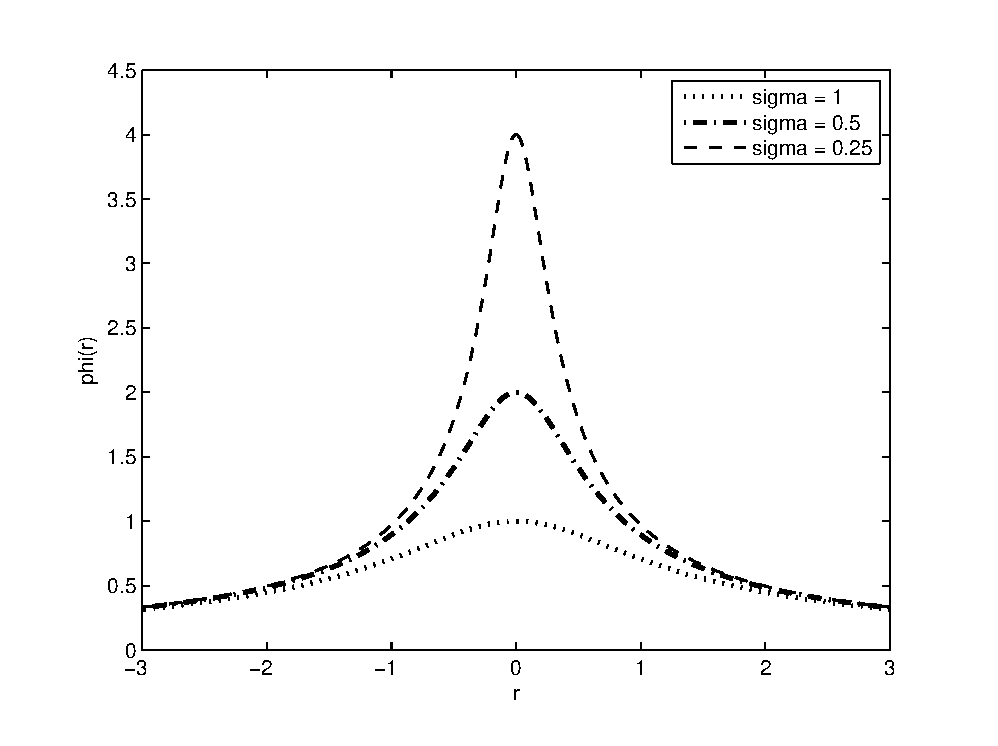
\includegraphics[width=0.8\columnwidth]{figures/nl_models_rbf.eps}
	\caption{Fun��o multiquadr�ticas inversa para alguns valores de $\sigma$.}
	\label{fig:nl_models_rbf}
\end{figure}

Este tipo de representa��o tem boas propriedades locais e pode ser interpretada como 
uma t�cnica de interpola��o global. Fun��es radiais de base s�o casos particulares
de redes neurais, porem neste caso lineares nos parametros $w_i$.\cite{aguirre} 

No contexto de identifica��o de sistemas � comum adicionar termos auto-regressivos
lineares, bem como termos de entrada � equa��o \eqref{eq:nl_models_rbf} resultando em:

\begin{equation}
y(k)=w_0 + \sum_{i}w_i \phi(\left \| \mathbf{y}(k-1)-c_i \right \|)+\sum_{i=1}^{n_y}a_i y(k-i)+\sum_{i=1}^{n_u}b_i u(k-i)+e(k)
\nonumber
\end{equation}

Sendo $\mathbf{y}(k-1)=\begin{bmatrix}
y(k-1) & ... & y(k-n_y) & u(k-1) & ... & u(k-n_u)
\end{bmatrix}$.

%===============================================================================
\section{Modelos NARMAX}
\label{sec:nl_models_narmax}
% Aguirre 343
%===============================================================================

Os modelos {\it{NARX}} (do termo ingles {\it{nonlinear autoregressive model with
exogenous variables}}) s�o modelos discretos no tempo que caracterizam o valor da 
sa�da em fun��o dos valor passados da entrada e sa�da. Algumas vezes, para evitar 
a polariza��o da estimativa dos parametros adiciona-se termos do ruido no modelo.
Quando isso � feito o modelo passa a ser chamado de um modelo {\it{NARMAX}} (do
termo ingles {\it{nonlinear autoregressive moving average model with exogenous
variables}}) que pode ser representado pla equa��o \eqref{eq:nl_model_narmax} 
\cite{aguirre}. Este modelo prov� uma representa��o unificada para a descri��o de sistemas discretos
n�o lineares \cite{chen_billings_narmax}

\begin{eqnarray}\nonumber
y(t)&=&F [ y(t-1), ..., y(t-n_y), u(t-1), ... , u(t-n_u),\\
&&  e(t),e(t-1), ... , e(t-n_e) ]
\label{eq:nl_model_narmax}
\end{eqnarray}

Onde $e(t)$ � o ruido e $n_e$ � o maior atraso no modelo do ruido. O modelo apresentado
em \eqref{eq:nl_model_narmax} � bastante gen�rico, caracterizando uma dificuldade 
para sua utiliza��o. A caracteriza��o da equa��o $F$ geralmente � feita pelas 
representa��es polinomial e racional. Um modelo polinomial {\it{NARMAX}} sem atraso
puro de tempo tem a forma apresentada em \eqref{eq:nl_model_narmax_pol}.

\begin{equation}
y(t)=\sum_{i}c_i \prod_{j=1}^{n_y}y(t-j) \prod_{r=1}^{n_u}u(t-r) \prod_{q=0}^{n_e}e(t-q)
\label{eq:nl_model_narmax_pol}
\end{equation}

Os modelos polinomiais {\it{bilineares}} s�o casos particulares do modelo polinomial 
\eqref{eq:nl_model_narmax_pol} quando todos os termos n�o lineares s�o do tipo 
$y(t-i)u(t-j), \; \forall i,j$. \cite{aguirre}

Modelos racionais s�o formados pela raz�o entre dois polinomios \eqref{eq:nl_model_narmax_rat}.

\begin{equation}
y(t)=\frac{\sum_{i}c_i \prod_{j=1}^{n_y}y(t-j) \prod_{r=1}^{n_u}u(t-r) \prod_{q=0}^{n_e}e(t-q)}
{\sum_{i}c_i \prod_{j=1}^{n_y}y(t-j) \prod_{r=1}^{n_u}u(t-r) \prod_{q=0}^{n_e}e(t-q)} + e(t)
\label{eq:nl_model_narmax_rat}
\end{equation}

Em fun��o de terem uma estrutura mais floxivel, os modelos racionais opdem vir a ser
mais eficientes na modelagem de certos sistemas quando comparados com modelos polinomiais.
Entretanto, os modelos racionais s�o mais sens�veis ao ruido. \cite{aguirre}

%===============================================================================
\subsection{Modelo polinomial}
\label{sec:nl_models_narmax_pol}
% Aguirre 343
%===============================================================================
Com rela��o ao modelo generico polinomial {\it{NARMAX}} apresentado em \eqref{eq:nl_model_narmax_pol}
duas considera��es ser�o levadas em conta:

\begin{enumerate}
\item O sistema tem um atraso puro de tempo $\tau _d$ 
\item Nenhum termo cujo parametro tenha que ser estimado pode depender de $e(t)$.
\end{enumerate}

A segunda considera��o implica em tornar $F$ independente de $e(t)$. O que equivale a dizer
que $q=1$ em \eqref{eq:nl_model_narmax_pol} resultando em  \eqref{eq:nl_model_narmax_pol_espec}.

\begin{eqnarray}\nonumber
y(t) &=& F[ y(t-1), ..., y(t-n_y), u(t-\tau_d), ..., u(t-\tau_d-n_u+1),\\
&& e(t-1), ..., e(t-n_e)] +e(t)
\label{eq:nl_model_narmax_pol_espec}
\end{eqnarray}

Sendo que $e(t)$ indica que todos os efeitos n�o podem ser bem representados por 
$F^l\left [ \cdot  \right ]$, � uma fun��o polinomial de $y(t)$, $u(t)$ e 
$e(t)$ com grau de n�o linearidade $l\in \mathbb{N}$. Portanto a parte 
n�o deterministica de \eqref{eq:nl_model_narmax_pol_espec} pode ser espandida como
um somat�rio de termos com grau de n�o linearidade variando de $1 \le m \le l$. 
Assim sendo, cada termo de grau $m$ poder� conter um falor de grau $p$ do tipo $y(t-i)$
e um fator de grau $(m-p)$ do tipo $u(t-i)$ sendo multiplicado por um parametro representado 
por $c_{p,m-p}(n_1, ..., n_m$. Resultando em: \cite{aguirre}

\begin{equation}
y(t)=\sum_{m=0}^{l}\sum_{p=0}^{m}\sum_{n1, n_m}^{n_y, n_u}c_{p,m-p}(n_1,...,n_m)\prod_{i=1}^{p}y(t-n_i)\prod_{i=p+1}^{m}u(t-n_i)
\nonumber
\end{equation}


%===============================================================================
\subsection{Modelo Racional}
\label{sec:nl_models_narmax_rat}
% Aguirre 345
%===============================================================================

Um modelo racional {\it{NARMAX}} tem a seguinte forma geral apresentada em 
\eqref{eq:nl_model_narmax_rat} e de forma simplificada como apresentado em
\eqref{eq:nl_model_narmax_rat_simp}.

\begin{equation}
y(k)=\frac{a(\Upsilon)}{b(\Upsilon)}+e(t)
\label{eq:nl_model_narmax_rat_simp}
\end{equation}

Onde:

\begin{equation}
\Upsilon=\left \{ y(t-1), ..., y(t-n_y), u(t-1), ..., u(t-n_u), e(t-1), ..., e(t-n_e)\right \}
\nonumber
\end{equation}

No modelo apresentado em \eqref{eq:nl_model_narmax_rat}, as fun��es $a(\Upsilon)$ e $b(\Upsilon)$
s�o polinomios, mas poderiam ser quaisquer fun��es. Assumindo que o modelo � formado pela raz�o de
dois polinomios, � conveniente definir o numerador e denominador de \eqref{eq:nl_model_narmax_rat}
como em \eqref{eq:nl_model_narmax_rat_num} e \eqref{eq:nl_model_narmax_rat_den}

\begin{equation}
a(t-1)=\sum_{j=1}^{N_n}p_{nj}\theta_{nj}=\psi _n^T(k-1)\theta_n
\label{eq:nl_model_narmax_rat_num}
\end{equation}


\begin{equation}
b(t-1)=\sum_{j=1}^{N_d}p_{dj}\theta_{dj}=\psi _d^T(k-1)\theta_d
\label{eq:nl_model_narmax_rat_den}
\end{equation}

Sendo $\theta_{nj}$ e $\theta_{dj}$ s�o os parametros dos regressores, possuindo informa��es at� o
instante $t-1$. Desta forma o valor de parametros a ser estimados � $N_n + N_d$

A equa��o \eqref{eq:nl_model_narmax_rat_simp} possui n�o linearidade nos parametros, tornando a
identifica��o mais complexa por n�o ser poss�vel utilizar o m�todo dos minimos quadrados para a
estimativa dos parametros. Uma alternativa para este problema � multiplicar a equa��o
\eqref{eq:nl_model_narmax_rat_simp} pela equa��o \eqref{eq:nl_model_narmax_rat_den} em ambos os seus
lados. \cite{billings_zhu91}

\begin{equation}
Y(t)=a(t)-y(t)\sum_{j=2}^{den}p_{dj}(t)\theta_{dj}+b(t)e(t)
\nonumber
\end{equation}


\begin{equation}
Y(t)=\sum_{j=1}^{num}p_{nj}(t)\theta_{nj}-\sum_{j=2}^{den}y(t)p_{dj}(t)\theta_{dj}+\xi (t)
\label{eq:nl_model_narmax_rat_linear_param}
\end{equation}

Onde:

\begin{equation}
Y(t)=y(t)p_{d1}\mid_{\theta_{d1}=1} =p_{d1}(t)\frac{a(t)}{b(t)}+p_{d1}(t)e(t)
\nonumber
\end{equation}

e

\begin{equation}
\xi(t)=b(t)e(t)=\left ( \sum_{j=1}^{den}p_{dj}(t)\theta_{dj} \right )e(t)
\nonumber
\end{equation}

Pelo fato de $e(t)$ ser independente de $b(t)$ e ter m�dia nula, tem-se:

\begin{equation}
E\left [ \xi(t) \right ]=E\left [ b(t) \right ]E\left [ e(t) \right ]=0
\label{eq:nl_model_narmax_rat_noise_var}
\end{equation}

A equa��o \eqref{nl_model_narmax_rat_linear_param} mostra que todos os termos $t(t)p_{dj}(t)$
incluem o termo de ruido $e(t)$ atrav�s de $y(t)$ que este por sua vez � altamente relacionado com
$\xi(t)$, o que resultar� em polariza��o dos parametros, mesmo que $e(t)$ seja um ruido branco com
m�dia zero. Este � de certa forma o pre�o que se paga ao linearizar os parametros e ser poss�vel
utilizar o m�todo dos minimos quadrados. \cite{aguirre}

%===============================================================================
\subsubsection{Estimador usando m�todos dos minimos quadrados}
\label{sec:nl_models_narmax_rat_lsm}
% correa 31 - billings e zhu 1991
%===============================================================================



%===============================================================================
\section{Algoritmos para identifica��o}
\label{sec:nl_si_algorithms}
%===============================================================================

%===============================================================================
\subsection{Modelos Racionais}
\label{sec:nl_si_algorithms_rationals}
% Aguirre 393
% Tese do corr�a - pg 27
%===============================================================================

\input{tex/chapters/nlin_si_conclusions}
%===============================================================================

